% This is the Duke University Statistical Science LaTeX thesis template.
% It has been adapted from the Reed College LaTeX thesis template. The
% adaptation was done by Mine Cetinkaya-Rundel (MCR). Some of the comments
% that are specific to Reed College have been removed.
%
% Most of the work on the original Reed College document class and template
% was done by Sam Noble (SN). Later comments etc. by Ben Salzberg (BTS).
% Additional restructuring and APA support by Jess Youngberg (JY).
%
% See https://www.reed.edu/cis/help/latex/ for help. There are a
% great bunch of help pages there, with notes on
% getting started, bibtex, etc. Go there and read it if you're not
% already familiar with LaTeX.
%
% Any line that starts with a percent symbol is a comment.
% They won't show up in the document, and are useful for notes
% to yourself and explaining commands.
% Commenting also removes a line from the document;
% very handy for troubleshooting problems. -BTS

%%
%% Preamble
%%
% \documentclass{<something>} must begin each LaTeX document
\documentclass[12pt,twoside]{dukestatscithesis}
% Packages are extensions to the basic LaTeX functions. Whatever you
% want to typeset, there is probably a package out there for it.
% Chemistry (chemtex), screenplays, you name it.
% Check out CTAN to see: http://www.ctan.org/
%%
\usepackage{graphicx,latexsym}
\usepackage{amsmath}
\usepackage{amssymb,amsthm}
\usepackage{longtable,booktabs,setspace}
\usepackage{chemarr} %% Useful for one reaction arrow, useless if you're not a chem major
\usepackage[hyphens]{url}
% Added by CII
\usepackage{hyperref}
\usepackage{lmodern}
\usepackage{float}
\floatplacement{figure}{H}
% End of CII addition
\usepackage{rotating}

% Next line commented out by CII
%%% \usepackage{natbib}
% Comment out the natbib line above and uncomment the following two lines to use the new
% biblatex-chicago style, for Chicago A. Also make some changes at the end where the
% bibliography is included.
%\usepackage{biblatex-chicago}
%\bibliography{thesis}


% Added by CII (Thanks, Hadley!)
% Use ref for internal links
\renewcommand{\hyperref}[2][???]{\autoref{#1}}
\def\chapterautorefname{Chapter}
\def\sectionautorefname{Section}
\def\subsectionautorefname{Subsection}
% End of CII addition

% Added by CII
\usepackage{caption}
\captionsetup{width=5in}
% End of CII addition

% \usepackage{times} % other fonts are available like times, bookman, charter, palatino


% To pass between YAML and LaTeX the dollar signs are added by CII
\title{Stochastic Process Model with Basketball Data}
\author{Sonia Xu}
% The month and year that you submit your FINAL draft TO THE LIBRARY (May or December)
\date{October 2017}
\advisor{Dr.~Alexander Volfovsky}
\institution{Duke University}
\degree{Bachelor of Science in Statistical Science}
\committeememberone{Committeemember O. Name}
\committeemembertwo{Committeemember T. Name}
\dus{Dus X. Name}
%If you have two advisors for some reason, you can use the following
% Uncommented out by CII
% End of CII addition

%%% Remember to use the correct department!
\department{Department of Statistical Science}

% Added by CII
%%% Copied from knitr
%% maxwidth is the original width if it's less than linewidth
%% otherwise use linewidth (to make sure the graphics do not exceed the margin)
\makeatletter
\def\maxwidth{ %
  \ifdim\Gin@nat@width>\linewidth
    \linewidth
  \else
    \Gin@nat@width
  \fi
}
\makeatother

\renewcommand{\contentsname}{Table of Contents}
% End of CII addition

\setlength{\parskip}{0pt}

% Added by CII

\providecommand{\tightlist}{%
  \setlength{\itemsep}{0pt}\setlength{\parskip}{0pt}}

\Acknowledgements{
I want to thank a few people.
}

\Dedication{
You can have a dedication here if you wish.
}

\Preface{
This is an example of a thesis setup to use the reed thesis document
class (for LaTeX) and the R bookdown package, in general.
}

\Abstract{
The preface pretty much says it all. \par

Second paragraph of abstract starts here.
}

% End of CII addition
%%
%% End Preamble
%%
%

\usepackage{amsthm}
\newtheorem{theorem}{Theorem}[chapter]
\newtheorem{lemma}{Lemma}[chapter]
\theoremstyle{definition}
\newtheorem{definition}{Definition}[chapter]
\newtheorem{corollary}{Corollary}[chapter]
\newtheorem{proposition}{Proposition}[chapter]
\theoremstyle{definition}
\newtheorem{example}{Example}[chapter]
\theoremstyle{definition}
\newtheorem{exercise}{Exercise}[chapter]
\theoremstyle{remark}
\newtheorem*{remark}{Remark}
\newtheorem*{solution}{Solution}
\begin{document}

% Everything below added by CII
  \maketitle

\frontmatter % this stuff will be roman-numbered
\pagestyle{empty} % this removes page numbers from the frontmatter
  \begin{acknowledgements}
    I want to thank a few people.
  \end{acknowledgements}
  \begin{preface}
    This is an example of a thesis setup to use the reed thesis document
    class (for LaTeX) and the R bookdown package, in general.
  \end{preface}
  \hypersetup{linkcolor=black}
  \setcounter{tocdepth}{2}
  \tableofcontents

  \listoftables

  \listoffigures
  \begin{abstract}
    The preface pretty much says it all. \par
    
    Second paragraph of abstract starts here.
  \end{abstract}
  \begin{dedication}
    You can have a dedication here if you wish.
  \end{dedication}
\mainmatter % here the regular arabic numbering starts
\pagestyle{fancyplain} % turns page numbering back on

\chapter{thesisdowndss::thesis\_word:
default}\label{thesisdowndssthesis_word-default}

\chapter{Boxscore}\label{boxscore}

In basketball, a boxscore provides the statistical summary of the game
via defensive, offensive, and overall success metrics. Popular metrics
include rebounds per game (RBG), player efficiency rating (PER), free
throw attempts (FTA), and 3 field goals made (3FGM). However, these
metrics cannot capture the entirety of the game because they do not take
into account the opposing team's defense/offense, nor previous plays
that significantly influenced the flow of the game.

\chapter{Literature Review}\label{rmd-basics}

Previous works have sought to capture the game more robustly. Below
describes a summary of a few:

``Flow Motifs in Soccer: What can passing behavior tell us?'' by Joris
Bekkers and Shaunak Dabadghao was released in the 2017 MIT Sloan Sports
Analytics Conference, and focused on the static passing networks of
``the last 4 seasons of 6 big European leagues with 8219 matches, 3532
unique players and 155 unique teams.'' Passing sequences were denoted as
a sequence of all players involved five seconds before an attempted
score. This paper created radar graphs that illustrated the most popular
passing sequences by player, and compared radar graphs to identify
similar players. Passing sequences within teams were also compared
between teams by clustering the different passing styles of the
different teams. Key players were determined by the frequency that they
were included in the passing sequences.

``Exploring Team Passing Networks and Player Movement Dynamics in Youth
Association Football (Soccer)'' by Bruno Goncalves, Diogo Coutinho, Sara
Santos, Carlos Lago-Penas, Sergio Jimenez, and Jamie Sampaio compared
the passing sequences of two games played by two groups that differ in
age range, which showed that regardless of age, network centrality was
distinctive in both groups, and affirmed the long-held belief that more
passes lead to better game outcomes. Similar to the first paper, key
players were the ones most frequently involved in the passing sequences.
This paper created weighted graphs of the passing sequences, which
better visualized the passing structure of the team, and made it easier
to identify important players.

``Basketball Teams as Strategic Networks'' by Jennifer H. Fewell, Dieter
Armbruster, John Ingraham, Alexander Petersen, and James S. Waters
provided measurements to assess team entropy. First recording the
complete 30 seconds of a possession as a passing sequence, they
discovered that recording the last three nodes (players) before a shot
attempt was a better way to record passing sequences to avoid ``noisy''
passing data. Although they were able to recognize various aspects of
team dynamics through weighted graphs like the second paper, they did
not find a consistent predictor of positive game outcomes. This paper
also identified that in general, teams typically range between two
playing styles: always passing to the best player or having no distinct
patterns in passing. These patterns can be noted by distinct betweenness
scores and uniform betweenness scores, respectively. Weighted graphs
clearly illustrated the two different playing styles. Also, the paper
found that the positions most involved with successful shots were: 1. PG
2. SG 3. SF 4. PF 5. CN.

Joachim Gudmundsson and Michael Horton summarised a variety of methods
that utilize object tracking data to analyze team and player
performances in ``Spatio-Temporal Analysis of Team Sports -- A Survey.''
Their research survey spanned modeling passing networks via graph theory
to calculating rebound probability with spatial coordinates. In
particular, work conducted by Daniel Cervone, Alex D'Amour, Luke Bornn,
and Kirk Goldsberry attempted to capture the game wholelistically via a
new measure called Expected Possession Value (EPV) in the paper ``A
Multiresolution Stochastic Process Model for Predicting Basketball
Possession Outcomes.'' This new metric uses three models--a
Microtransition Model, Macrotransition Entrance Model, and a
Macrotransition Exit Model--to capture the spatial biases of each player
and the in-game effects of pressure, so that it can measure the
likelihood of a successful play (made shot) given the previous sequence
of events. To compare players against the league-average scores, they
also calculated Expected Possession Value -Adjusted as an application
for teams.

\chapter{Model Replication}\label{model-replication}

\section{Motivation}\label{motivation}

This paper is particularly interesting because EPV utilizes the
spatio-temporal elements of the game, so it models the NBA game
dynamically. Given Duke Basketball data, the motivation is to replicate
``A Multiresolution Stochastic Process Model for Predicting Basketball
Possession Outcomes,'' to better understand the Duke Men's team, as well
as to compare professional basketball to collegiate basketball
individual and team playing styles. Below is a brief overview of each
model used in the paper to calculate EPV.

\section{Microtransition Model}\label{microtransition-model}

\(x^{l}(t+\epsilon) = x^{l}(t) + \alpha^{l}_{x}[x^{l}(t) - x^{l}(t-\epsilon)] + \eta^{l}_{x}(t)\)
where
\(\eta^{l}_{x}(t) \sim N(\mu^{l}_{x}(z^{l}(t)), (\sigma^{l}_{x})^{2})\)

The microtransition model models the defensive conditions of the game
based on the \((x,y)\) coordinates of a player and their acceleration
effects (\(\alpha^{l}_{x}(t)\)). It is also assumed that a player's
spatial location is normally distributed. Since players play
differently, each microtransition model is specifically fitted to the
player.

\section{Macrotransition Entrance
Model}\label{macrotransition-entrance-model}

\(P(M(t)|F_{t}^{(Z)}\) The macrotransition entrance model predicts
whether the next move will be a pass (4 options), shot attempt, or
turnover. The model is disjoint.

\section{Macrotransition Exit Model}\label{macrotransition-exit-model}

\(P(C_{\delta_{t}}|M(t), F_{t}^{(Z)})\) Given the Macrotransition
Entrance Model predicts a shot attempt, it indexes to a logistic
regression model to calculate player \(l\)'s successful shot
probability. Given the Macrotransition Entrance Model predicts a pass,it
indexes to a model that predicts where the pass will take place.
Otherwise, a turnover is assumed.

\chapter{Macrotransition Exit Model}\label{macrotransition-exit-model-1}

\(equation\)

\chapter{Implementation of this
Model}\label{implementation-of-this-model}

\section{in the works\ldots{}}\label{in-the-works}

\section{Next Steps (have yet to get this
far)}\label{next-steps-have-yet-to-get-this-far}

Both metrics calculated via a semi-Markov process, EPV fails to capture
the full nature of the possession because it only uses the last
posession as a prior. The model would be more robust if it captured the
entirety of the posession in its prior--however, the computational time
of such an ordeal would prevent any real-time analyses. Thus, this paper
proposes that a simpler model may perform more quickly and potentially
just as robustly to allow for game-time analyses.

Here is a brief introduction into using \emph{R Markdown}.
\emph{Markdown} is a simple formatting syntax for authoring HTML, PDF,
and MS Word documents. \emph{R Markdown} provides the flexibility of
\emph{Markdown} with the implementation of \textbf{R} input and output.
For more details on using \emph{R Markdown} see
\url{http://rmarkdown.rstudio.com}.

Be careful with your spacing in \emph{Markdown} documents. While
whitespace largely is ignored, it does at times give \emph{Markdown}
signals as to how to proceed. As a habit, try to keep everything left
aligned whenever possible, especially as you type a new paragraph. In
other words, there is no need to indent basic text in the Rmd document
(in fact, it might cause your text to do funny things if you do).

\section{Exploratory Data Analysis}\label{exploratory-data-analysis}

-eda, write up literature

It's easy to create a list. It can be unordered like
\begin{itemize}
\tightlist
\item
  Item 1
\item
  Item 2
\end{itemize}
or it can be ordered like
\begin{enumerate}
\def\labelenumi{\arabic{enumi}.}
\tightlist
\item
  Item 1
\item
  Item 2
\end{enumerate}
Notice that I intentionally mislabeled Item 2 as number 4.
\emph{Markdown} automatically figures this out! You can put any numbers
in the list and it will create the list. Check it out below.

To create a sublist, just indent the values a bit (at least four spaces
or a tab). (Here's one case where indentation is key!)
\begin{enumerate}
\def\labelenumi{\arabic{enumi}.}
\tightlist
\item
  Item 1
\item
  Item 2
\item
  Item 3
  \begin{itemize}
  \tightlist
  \item
    Item 3a
  \item
    Item 3b
  \end{itemize}
\end{enumerate}
\section{Line breaks}\label{line-breaks}

Make sure to add white space between lines if you'd like to start a new
paragraph. Look at what happens below in the outputted document if you
don't:

Here is the first sentence. Here is another sentence. Here is the last
sentence to end the paragraph. This should be a new paragraph.

\emph{Now for the correct way:}

Here is the first sentence. Here is another sentence. Here is the last
sentence to end the paragraph.

This should be a new paragraph.

\section{R chunks}\label{r-chunks}

When you click the \textbf{Knit} button above a document will be
generated that includes both content as well as the output of any
embedded \textbf{R} code chunks within the document. You can embed an
\textbf{R} code chunk like this (\texttt{cars} is a built-in \textbf{R}
dataset):
\begin{Shaded}
\begin{Highlighting}[]
\KeywordTok{summary}\NormalTok{(cars)}
\end{Highlighting}
\end{Shaded}
\begin{verbatim}
     speed           dist       
 Min.   : 4.0   Min.   :  2.00  
 1st Qu.:12.0   1st Qu.: 26.00  
 Median :15.0   Median : 36.00  
 Mean   :15.4   Mean   : 42.98  
 3rd Qu.:19.0   3rd Qu.: 56.00  
 Max.   :25.0   Max.   :120.00  
\end{verbatim}
\section{Inline code}\label{inline-code}

If you'd like to put the results of your analysis directly into your
discussion, add inline code like this:
\begin{quote}
The \texttt{cos} of \(2 \pi\) is 1.
\end{quote}
Another example would be the direct calculation of the standard
deviation:
\begin{quote}
The standard deviation of \texttt{speed} in \texttt{cars} is 5.2876444.
\end{quote}
One last neat feature is the use of the \texttt{ifelse} conditional
statement which can be used to output text depending on the result of an
\textbf{R} calculation:
\begin{quote}
The standard deviation is less than 6.
\end{quote}
Note the use of \texttt{\textgreater{}} here, which signifies a
quotation environment that will be indented.

As you see with \texttt{\$2\ \textbackslash{}pi\$} above, mathematics
can be added by surrounding the mathematical text with dollar signs.
More examples of this are in {[}Mathematics and Science{]} if you
uncomment the code in \protect\hyperlink{math}{Math}.

\section{Including plots}\label{including-plots}

You can also embed plots. For example, here is a way to use the base
\textbf{R} graphics package to produce a plot using the built-in
\texttt{pressure} dataset:

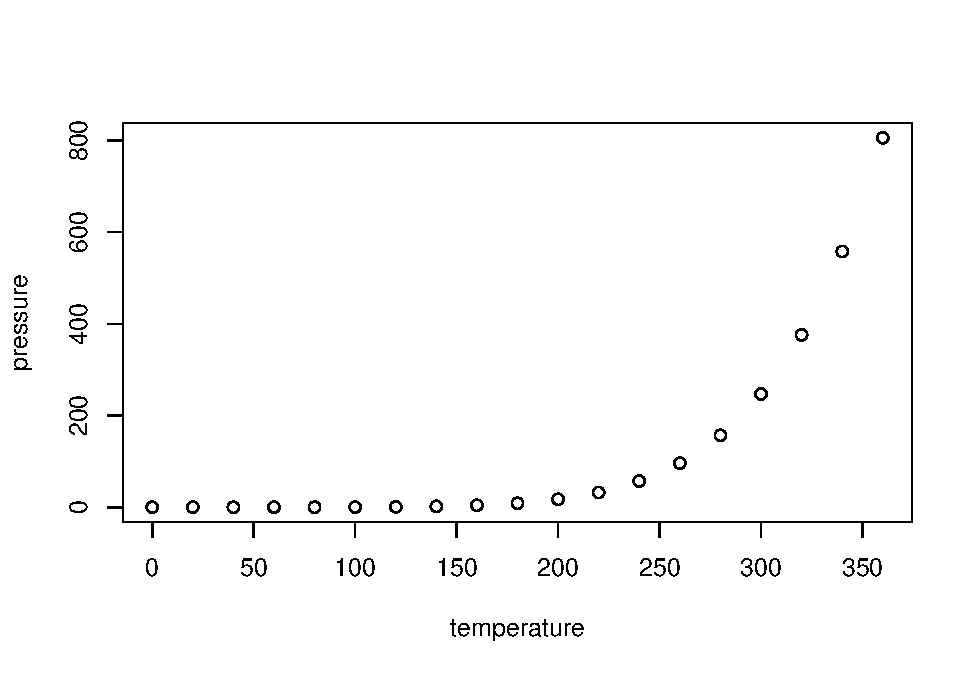
\includegraphics{thesis_files/figure-latex/pressure-1.pdf}

Note that the \texttt{echo=FALSE} parameter was added to the code chunk
to prevent printing of the \textbf{R} code that generated the plot.
There are plenty of other ways to add chunk options. More information is
available at \url{http://yihui.name/knitr/options/}.

Another useful chunk option is the setting of \texttt{cache=TRUE} as you
see here. If document rendering becomes time consuming due to long
computations or plots that are expensive to generate you can use knitr
caching to improve performance. Later in this file, you'll see a way to
reference plots created in \textbf{R} or external figures.

\section{Loading and exploring data}\label{loading-and-exploring-data}

Included in this template is a file called \texttt{flights.csv}. This
file includes a subset of the larger dataset of information about all
flights that departed from Seattle and Portland in 2014. More
information about this dataset and its \textbf{R} package is available
at \url{http://github.com/ismayc/pnwflights14}. This subset includes
only Portland flights and only rows that were complete with no missing
values. Merges were also done with the \texttt{airports} and
\texttt{airlines} data sets in the \texttt{pnwflights14} package to get
more descriptive airport and airline names.

We can load in this data set using the following command:
\begin{Shaded}
\begin{Highlighting}[]
\NormalTok{flights <-}\StringTok{ }\KeywordTok{read.csv}\NormalTok{(}\StringTok{"data/flights.csv"}\NormalTok{)}
\end{Highlighting}
\end{Shaded}
The data is now stored in the data frame called \texttt{flights} in
\textbf{R}. To get a better feel for the variables included in this
dataset we can use a variety of functions. Here we can see the
dimensions (rows by columns) and also the names of the columns.
\begin{Shaded}
\begin{Highlighting}[]
\KeywordTok{dim}\NormalTok{(flights)}
\end{Highlighting}
\end{Shaded}
\begin{verbatim}
[1] 52808    16
\end{verbatim}
\begin{Shaded}
\begin{Highlighting}[]
\KeywordTok{names}\NormalTok{(flights)}
\end{Highlighting}
\end{Shaded}
\begin{verbatim}
 [1] "month"        "day"          "dep_time"     "dep_delay"   
 [5] "arr_time"     "arr_delay"    "carrier"      "tailnum"     
 [9] "flight"       "dest"         "air_time"     "distance"    
[13] "hour"         "minute"       "carrier_name" "dest_name"   
\end{verbatim}
Another good idea is to take a look at the dataset in table form. With
this dataset having more than 50,000 rows, we won't explicitly show the
results of the command here. I recommend you enter the command into the
Console \textbf{\emph{after}} you have run the \textbf{R} chunks above
to load the data into \textbf{R}.
\begin{Shaded}
\begin{Highlighting}[]
\KeywordTok{View}\NormalTok{(flights)}
\end{Highlighting}
\end{Shaded}
While not required, it is highly recommended you use the \texttt{dplyr}
package to manipulate and summarize your data set as needed. It uses a
syntax that is easy to understand using chaining operations. Below I've
created a few examples of using \texttt{dplyr} to get information about
the Portland flights in 2014. You will also see the use of the
\texttt{ggplot2} package, which produces beautiful, high-quality
academic visuals.

We begin by checking to ensure that needed packages are installed and
then we load them into our current working environment:
\begin{Shaded}
\begin{Highlighting}[]
\CommentTok{# List of packages required for this analysis}
\NormalTok{pkg <-}\StringTok{ }\KeywordTok{c}\NormalTok{(}\StringTok{"dplyr"}\NormalTok{, }\StringTok{"ggplot2"}\NormalTok{, }\StringTok{"knitr"}\NormalTok{, }\StringTok{"bookdown"}\NormalTok{, }\StringTok{"devtools"}\NormalTok{)}
\CommentTok{# Check if packages are not installed and assign the}
\CommentTok{# names of the packages not installed to the variable new.pkg}
\NormalTok{new.pkg <-}\StringTok{ }\NormalTok{pkg[}\OperatorTok{!}\NormalTok{(pkg }\OperatorTok\StringTok{ }\KeywordTok{installed.packages}\NormalTok{())]}
\CommentTok{# If there are any packages in the list that aren't installed,}
\CommentTok{# install them}
\ControlFlowTok{if}\NormalTok{ (}\KeywordTok{length}\NormalTok{(new.pkg))}
  \KeywordTok{install.packages}\NormalTok{(new.pkg, }\DataTypeTok{repos =} \StringTok{"http://cran.rstudio.com"}\NormalTok{)}
\CommentTok{# Load packages (thesisdowndss will load all of the packages as well)}
\KeywordTok{library}\NormalTok{(thesisdowndss)}
\end{Highlighting}
\end{Shaded}
\clearpage

The example we show here does the following:
\begin{itemize}
\item
  Selects only the \texttt{carrier\_name} and \texttt{arr\_delay} from
  the \texttt{flights} dataset and then assigns this subset to a new
  variable called \texttt{flights2}.
\item
  Using \texttt{flights2}, we determine the largest arrival delay for
  each of the carriers.
\end{itemize}
\begin{Shaded}
\begin{Highlighting}[]
\NormalTok{flights2 <-}\StringTok{ }\NormalTok{flights }\OperatorTok\StringTok{ }
\StringTok{  }\KeywordTok{select}\NormalTok{(carrier_name, arr_delay)}
\NormalTok{max_delays <-}\StringTok{ }\NormalTok{flights2 }\OperatorTok\StringTok{ }
\StringTok{  }\KeywordTok{group_by}\NormalTok{(carrier_name) }\OperatorTok
\StringTok{  }\KeywordTok{summarize}\NormalTok{(}\DataTypeTok{max_arr_delay =} \KeywordTok{max}\NormalTok{(arr_delay, }\DataTypeTok{na.rm =} \OtherTok{TRUE}\NormalTok{))}
\end{Highlighting}
\end{Shaded}
A useful function in the \texttt{knitr} package for making nice tables
in \emph{R Markdown} is called \texttt{kable}. It is much easier to use
than manually entering values into a table by copying and pasting values
into Excel or LaTeX. This again goes to show how nice reproducible
documents can be! (Note the use of \texttt{results="asis"}, which will
produce the table instead of the code to create the table.) The
\texttt{caption.short} argument is used to include a shorter title to
appear in the List of Tables.
\begin{Shaded}
\begin{Highlighting}[]
\KeywordTok{kable}\NormalTok{(max_delays, }
      \DataTypeTok{col.names =} \KeywordTok{c}\NormalTok{(}\StringTok{"Airline"}\NormalTok{, }\StringTok{"Max Arrival Delay"}\NormalTok{),}
      \DataTypeTok{caption =} \StringTok{"Maximum Delays by Airline"}\NormalTok{,}
      \DataTypeTok{caption.short =} \StringTok{"Max Delays by Airline"}\NormalTok{,}
      \DataTypeTok{longtable =} \OtherTok{TRUE}\NormalTok{,}
      \DataTypeTok{booktabs =} \OtherTok{TRUE}\NormalTok{)}
\end{Highlighting}
\end{Shaded}
\begin{longtable}[t]{lr}
\caption[Max Delays by Airline]{\label{tab:maxdelays}Maximum Delays by Airline}\\
\toprule
Airline & Max Arrival Delay\\
\midrule
Alaska Airlines Inc. & 338\\
American Airlines Inc. & 1539\\
Delta Air Lines Inc. & 651\\
Frontier Airlines Inc. & 575\\
Hawaiian Airlines Inc. & 407\\
\addlinespace
JetBlue Airways & 273\\
SkyWest Airlines Inc. & 421\\
Southwest Airlines Co. & 694\\
United Air Lines Inc. & 472\\
US Airways Inc. & 347\\
Virgin America & 366\\
\bottomrule
\end{longtable}
The last two options make the table a little easier-to-read.

We can further look into the properties of the largest value here for
American Airlines Inc. To do so, we can isolate the row corresponding to
the arrival delay of 1539 minutes for American in our original
\texttt{flights} dataset.
\begin{Shaded}
\begin{Highlighting}[]
\NormalTok{flights }\OperatorTok\StringTok{ }\KeywordTok{filter}\NormalTok{(arr_delay }\OperatorTok{==}\StringTok{ }\DecValTok{1539}\NormalTok{, }
\NormalTok{                  carrier_name }\OperatorTok{==}\StringTok{ "American Airlines Inc."}\NormalTok{) }\OperatorTok
\StringTok{  }\KeywordTok{select}\NormalTok{(}\OperatorTok{-}\KeywordTok{c}\NormalTok{(month, day, carrier, dest_name, hour, }
\NormalTok{            minute, carrier_name, arr_delay))}
\end{Highlighting}
\end{Shaded}
\begin{verbatim}
  dep_time dep_delay arr_time tailnum flight dest air_time distance
1     1403      1553     1934  N595AA   1568  DFW      182     1616
\end{verbatim}
We see that the flight occurred on March 3rd and departed a little after
2 PM on its way to Dallas/Fort Worth. Lastly, we show how we can
visualize the arrival delay of all departing flights from Portland on
March 3rd against time of departure.
\begin{Shaded}
\begin{Highlighting}[]
\NormalTok{flights }\OperatorTok\StringTok{ }\KeywordTok{filter}\NormalTok{(month }\OperatorTok{==}\StringTok{ }\DecValTok{3}\NormalTok{, day }\OperatorTok{==}\StringTok{ }\DecValTok{3}\NormalTok{) }\OperatorTok
\StringTok{  }\KeywordTok{ggplot}\NormalTok{(}\KeywordTok{aes}\NormalTok{(}\DataTypeTok{x =}\NormalTok{ dep_time, }\DataTypeTok{y =}\NormalTok{ arr_delay)) }\OperatorTok{+}\StringTok{ }\KeywordTok{geom_point}\NormalTok{()}
\end{Highlighting}
\end{Shaded}
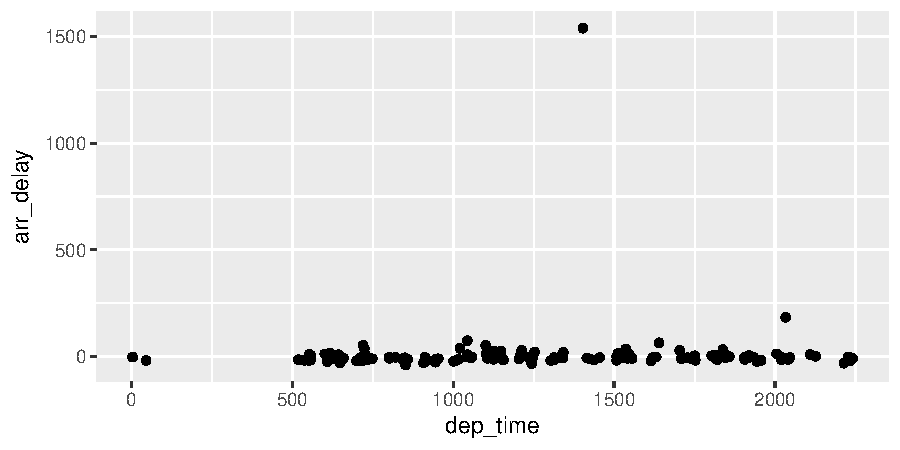
\includegraphics{thesis_files/figure-latex/march3plot-1.pdf}

\section{Additional resources}\label{additional-resources}
\begin{itemize}
\item
  \emph{Markdown} Cheatsheet -
  \url{https://github.com/adam-p/markdown-here/wiki/Markdown-Cheatsheet}
\item
  \emph{R Markdown} Reference Guide -
  \url{https://www.rstudio.com/wp-content/uploads/2015/03/rmarkdown-reference.pdf}
\item
  \texttt{dplyr} Documentation - \url{http://dplyr.tidyverse.org/}
\item
  \texttt{ggplot2} Documentation - \url{http://ggplot2.tidyverse.org/}
\end{itemize}
\hypertarget{math}{\chapter{Math typesetting}\label{math}}

\hypertarget{math}{\section{Math}\label{math}}

\chapter{This chunk ensures that the thesisdowndss package
is}\label{this-chunk-ensures-that-the-thesisdowndss-package-is}

\section{Tables}\label{tables}

\section{Figures}\label{figures}

\section{Footnotes and Endnotes}\label{footnotes-and-endnotes}

\section{Bibliographies}\label{bibliographies}

\section{Anything else?}\label{anything-else}

\chapter{Organization}\label{organization}

\chapter*{Conclusion}\label{conclusion}
\addcontentsline{toc}{chapter}{Conclusion}

\chapter{The First Appendix}\label{the-first-appendix}

\chapter*{References}\label{references}
\addcontentsline{toc}{chapter}{References}


% Index?

\end{document}
